\documentclass[]{book}
\usepackage{lmodern}
\usepackage{amssymb,amsmath}
\usepackage{ifxetex,ifluatex}
\usepackage{fixltx2e} % provides \textsubscript
\ifnum 0\ifxetex 1\fi\ifluatex 1\fi=0 % if pdftex
  \usepackage[T1]{fontenc}
  \usepackage[utf8]{inputenc}
\else % if luatex or xelatex
  \ifxetex
    \usepackage{mathspec}
  \else
    \usepackage{fontspec}
  \fi
  \defaultfontfeatures{Ligatures=TeX,Scale=MatchLowercase}
\fi
% use upquote if available, for straight quotes in verbatim environments
\IfFileExists{upquote.sty}{\usepackage{upquote}}{}
% use microtype if available
\IfFileExists{microtype.sty}{%
\usepackage{microtype}
\UseMicrotypeSet[protrusion]{basicmath} % disable protrusion for tt fonts
}{}
\usepackage[margin=1in]{geometry}
\usepackage{hyperref}
\hypersetup{unicode=true,
            pdftitle={BGuide - Cálculo 1},
            pdfauthor={Bruno Geronymo},
            pdfborder={0 0 0},
            breaklinks=true}
\urlstyle{same}  % don't use monospace font for urls
\usepackage{natbib}
\bibliographystyle{apalike}
\usepackage{color}
\usepackage{fancyvrb}
\newcommand{\VerbBar}{|}
\newcommand{\VERB}{\Verb[commandchars=\\\{\}]}
\DefineVerbatimEnvironment{Highlighting}{Verbatim}{commandchars=\\\{\}}
% Add ',fontsize=\small' for more characters per line
\usepackage{framed}
\definecolor{shadecolor}{RGB}{248,248,248}
\newenvironment{Shaded}{\begin{snugshade}}{\end{snugshade}}
\newcommand{\KeywordTok}[1]{\textcolor[rgb]{0.13,0.29,0.53}{\textbf{#1}}}
\newcommand{\DataTypeTok}[1]{\textcolor[rgb]{0.13,0.29,0.53}{#1}}
\newcommand{\DecValTok}[1]{\textcolor[rgb]{0.00,0.00,0.81}{#1}}
\newcommand{\BaseNTok}[1]{\textcolor[rgb]{0.00,0.00,0.81}{#1}}
\newcommand{\FloatTok}[1]{\textcolor[rgb]{0.00,0.00,0.81}{#1}}
\newcommand{\ConstantTok}[1]{\textcolor[rgb]{0.00,0.00,0.00}{#1}}
\newcommand{\CharTok}[1]{\textcolor[rgb]{0.31,0.60,0.02}{#1}}
\newcommand{\SpecialCharTok}[1]{\textcolor[rgb]{0.00,0.00,0.00}{#1}}
\newcommand{\StringTok}[1]{\textcolor[rgb]{0.31,0.60,0.02}{#1}}
\newcommand{\VerbatimStringTok}[1]{\textcolor[rgb]{0.31,0.60,0.02}{#1}}
\newcommand{\SpecialStringTok}[1]{\textcolor[rgb]{0.31,0.60,0.02}{#1}}
\newcommand{\ImportTok}[1]{#1}
\newcommand{\CommentTok}[1]{\textcolor[rgb]{0.56,0.35,0.01}{\textit{#1}}}
\newcommand{\DocumentationTok}[1]{\textcolor[rgb]{0.56,0.35,0.01}{\textbf{\textit{#1}}}}
\newcommand{\AnnotationTok}[1]{\textcolor[rgb]{0.56,0.35,0.01}{\textbf{\textit{#1}}}}
\newcommand{\CommentVarTok}[1]{\textcolor[rgb]{0.56,0.35,0.01}{\textbf{\textit{#1}}}}
\newcommand{\OtherTok}[1]{\textcolor[rgb]{0.56,0.35,0.01}{#1}}
\newcommand{\FunctionTok}[1]{\textcolor[rgb]{0.00,0.00,0.00}{#1}}
\newcommand{\VariableTok}[1]{\textcolor[rgb]{0.00,0.00,0.00}{#1}}
\newcommand{\ControlFlowTok}[1]{\textcolor[rgb]{0.13,0.29,0.53}{\textbf{#1}}}
\newcommand{\OperatorTok}[1]{\textcolor[rgb]{0.81,0.36,0.00}{\textbf{#1}}}
\newcommand{\BuiltInTok}[1]{#1}
\newcommand{\ExtensionTok}[1]{#1}
\newcommand{\PreprocessorTok}[1]{\textcolor[rgb]{0.56,0.35,0.01}{\textit{#1}}}
\newcommand{\AttributeTok}[1]{\textcolor[rgb]{0.77,0.63,0.00}{#1}}
\newcommand{\RegionMarkerTok}[1]{#1}
\newcommand{\InformationTok}[1]{\textcolor[rgb]{0.56,0.35,0.01}{\textbf{\textit{#1}}}}
\newcommand{\WarningTok}[1]{\textcolor[rgb]{0.56,0.35,0.01}{\textbf{\textit{#1}}}}
\newcommand{\AlertTok}[1]{\textcolor[rgb]{0.94,0.16,0.16}{#1}}
\newcommand{\ErrorTok}[1]{\textcolor[rgb]{0.64,0.00,0.00}{\textbf{#1}}}
\newcommand{\NormalTok}[1]{#1}
\usepackage{longtable,booktabs}
\usepackage{graphicx,grffile}
\makeatletter
\def\maxwidth{\ifdim\Gin@nat@width>\linewidth\linewidth\else\Gin@nat@width\fi}
\def\maxheight{\ifdim\Gin@nat@height>\textheight\textheight\else\Gin@nat@height\fi}
\makeatother
% Scale images if necessary, so that they will not overflow the page
% margins by default, and it is still possible to overwrite the defaults
% using explicit options in \includegraphics[width, height, ...]{}
\setkeys{Gin}{width=\maxwidth,height=\maxheight,keepaspectratio}
\IfFileExists{parskip.sty}{%
\usepackage{parskip}
}{% else
\setlength{\parindent}{0pt}
\setlength{\parskip}{6pt plus 2pt minus 1pt}
}
\setlength{\emergencystretch}{3em}  % prevent overfull lines
\providecommand{\tightlist}{%
  \setlength{\itemsep}{0pt}\setlength{\parskip}{0pt}}
\setcounter{secnumdepth}{5}
% Redefines (sub)paragraphs to behave more like sections
\ifx\paragraph\undefined\else
\let\oldparagraph\paragraph
\renewcommand{\paragraph}[1]{\oldparagraph{#1}\mbox{}}
\fi
\ifx\subparagraph\undefined\else
\let\oldsubparagraph\subparagraph
\renewcommand{\subparagraph}[1]{\oldsubparagraph{#1}\mbox{}}
\fi

%%% Use protect on footnotes to avoid problems with footnotes in titles
\let\rmarkdownfootnote\footnote%
\def\footnote{\protect\rmarkdownfootnote}

%%% Change title format to be more compact
\usepackage{titling}

% Create subtitle command for use in maketitle
\newcommand{\subtitle}[1]{
  \posttitle{
    \begin{center}\large#1\end{center}
    }
}

\setlength{\droptitle}{-2em}
  \title{BGuide - Cálculo 1}
  \pretitle{\vspace{\droptitle}\centering\huge}
  \posttitle{\par}
  \author{Bruno Geronymo}
  \preauthor{\centering\large\emph}
  \postauthor{\par}
  \predate{\centering\large\emph}
  \postdate{\par}
  \date{2018-03-06}

\usepackage{booktabs}
\usepackage{amsthm}
\makeatletter
\def\thm@space@setup{%
  \thm@preskip=8pt plus 2pt minus 4pt
  \thm@postskip=\thm@preskip
}
\makeatother
\usepackage[brazil]{babel}

\begin{document}
\maketitle

{
\setcounter{tocdepth}{1}
\tableofcontents
}
\chapter*{Prefácio}\label{prefacio}
\addcontentsline{toc}{chapter}{Prefácio}

Este material trata-se de um manual de resoluções dos exercícios
propostos no livro \emph{Um Curso de Cálculo, Volume 1, 5ª Edição} de
\emph{Hamilton Luiz Guidorizzi}. Ao decorrer das resoluções o material
busca apresentar, adicionalmente, resoluções computacionais através do
software \href{https://www.r-project.org/}{R de computação estatística}
para facilitar a visualização do problema e também o aprendizado da
linguagem \emph{R}.

O material procura abordar todos os assuntos tratados no livro do
\emph{Guidorizzi}, seguindo também a mesma ordem dos capítulos, para
facilitar a dinâmica de pesquisa por assuntos específicos.

\chapter{Números reais}\label{numeros-reais}

\section{Os Números Racionais}\label{os-numeros-racionais}

Por uma questão de notação admitiremos aqui que, sendo \(r\) um número
racional, se \(r \leqslant 0\), dizemos que \(r\) é não positivo. Da
mesma forma, se \(r \geqslant 0\), dizemos que \(r\) é não negativo.

Vale acrescentar aqui algumas definições que poderão auxiliar na leitura
do livro.

\begin{itemize}
\tightlist
\item
  \textbf{Abscissa}: Trata-se da coordenada de um ponto sobre uma reta.
\item
  \textbf{Irredutível}: Algo que não se pode reduzir. Uma fração é dita
  irredutível quando está em sua forma mais reduzida possível.
\end{itemize}

\section{Os Números Reais}\label{os-numeros-reais}

\textbf{EXEMPLO 4.} \emph{(Página 6)} Suponha \(x \geqslant 0\) e
\(y \geqslant 0\). Prove:

\begin{enumerate}
\def\labelenumi{\alph{enumi})}
\setcounter{enumi}{1}
\tightlist
\item
  \(x \leqslant y \Rightarrow x^{2} \leqslant y^{2}\).
\end{enumerate}

~~~~~~\emph{Resolução}:

\[\textrm{e} \ \left.\begin{matrix} 0 \leqslant x \leqslant y\\ 0 \leqslant x \leqslant y \end{matrix}\right\} \overset{(OM)}{\Rightarrow} \ \textrm{e} \ \left.\begin{matrix} xx \leqslant xy \\ xy \leqslant yy \end{matrix}\right\} \overset{(O3)}{\Rightarrow} xx \leqslant xy \leqslant yy \Rightarrow xx \leqslant yy \Rightarrow x^{2} \leqslant y^{2}\]

~

\begin{Shaded}
\begin{Highlighting}[]
\CommentTok{# Estudo por simulação:}

\NormalTok{##  Semente:}
\KeywordTok{set.seed}\NormalTok{(}\KeywordTok{sum}\NormalTok{(}\KeywordTok{utf8ToInt}\NormalTok{(}\StringTok{"BGuide"}\NormalTok{)))}

\NormalTok{##  Quantidade de números a serem gerados:}
\NormalTok{n <-}\StringTok{ }\DecValTok{1000000}

\NormalTok{##  Gera-se aqui 'n' números aleatórios seguindo a distribuição Uniforme de}
\NormalTok{## parâmetros 'min = 0' e 'max = 1':}
\NormalTok{x <-}\StringTok{ }\KeywordTok{runif}\NormalTok{(n)}

\NormalTok{##  Em seguida geramos mais 'n' números aleatórios seguindo uma distribuição}
\NormalTok{## Uniforme de parâmetros 'min = x' e 'max = 1'. Isto faz com que todos os}
\NormalTok{## números armazenados em y[i] sejam maiores do que os armazenados em x[i], com}
\NormalTok{## 'i' variando de 1 a 'n'. Mas não implica que y[i] seja maior do que x[j] com}
\NormalTok{## 'j' também variando de 1 a 'n' e 'i != j':}
\NormalTok{y <-}\StringTok{ }\KeywordTok{runif}\NormalTok{(n, }\DataTypeTok{min =}\NormalTok{ x)}

\NormalTok{##  Soma a quantidade de verificações onde a afirmação 'x^2 <= y^2' for}
\NormalTok{## verdadeira:}
\KeywordTok{sum}\NormalTok{(x}\OperatorTok{^}\DecValTok{2} \OperatorTok{<=}\StringTok{ }\NormalTok{y}\OperatorTok{^}\DecValTok{2}\NormalTok{)}
\end{Highlighting}
\end{Shaded}

\begin{verbatim}
## [1] 1000000
\end{verbatim}

\begin{Shaded}
\begin{Highlighting}[]
\NormalTok{##  Observe que o resultado é 1.000.000, exatamente a quantidade de números}
\NormalTok{## uniformes no intervalo (0, 1) que foram gerados. Logo para todas as}
\NormalTok{## simulações obteve-se 'x^2 <= y^2'.}

\NormalTok{##  Obs.: O resultado obtido por simulação não prova a propriedade acima, apenas}
\NormalTok{## cria evidências a favor dela. A simulação não é necessária aqui pois a}
\NormalTok{## propriedade pode ser provada analiticamente.}
\end{Highlighting}
\end{Shaded}

~

\textbf{EXEMPLO 9.} \emph{(Página 10)} Resolva a inequação
\(\frac{3x-1}{x+2} \geqslant 5\).

Sendo \(x < 2\):

\[\frac{3x-1}{x+2} \geqslant 5 \Leftrightarrow 3x-1 \leqslant 5(x+2).\]

Então o autor pergunta: Por quê?

Sabemos que \(1 < 2\), se multiplicássemos esta expressão por \(-1\) sem
alterarmos o sentido da desigualdade teríamos \(-1 < -2\) e sabemos que
esta afirmação não é verdadeira. Considerando \(a < 0\), se
multiplicarmos uma desigualdade por \(a\) altera-se o sentido da
desigualdade pois refletimos estes valores para o outro lado de um eixo
com relação a origem a uma taxa de progressão \(\left | a \right |\).
Porém, ao realizar este processo a direção de crescimento das unidades
permanece a mesma (não é refletida).

~

\begin{Shaded}
\begin{Highlighting}[]
\CommentTok{# Exemplo gráfico}

\NormalTok{##  O gráfico a seguir tem como objetivo a visualização do que foi dito}
\NormalTok{## anteriormente. Nele pode-se observar a propriedade 'x <= y  ==>  ky <= kx'}
\NormalTok{## quando 'k < 0'. No exemplo utilizaremos 'x = 2', 'y = 3' e 'k = -2'.}

\NormalTok{##  Cria um vetor dos valores a serem plotados:}
\NormalTok{xy <-}\StringTok{ }\KeywordTok{c}\NormalTok{(}\DecValTok{2}\NormalTok{, }\DecValTok{3}\NormalTok{)}
\NormalTok{k <-}\StringTok{ }\OperatorTok{-}\DecValTok{2}
\NormalTok{pontos <-}\StringTok{ }\KeywordTok{c}\NormalTok{(k}\OperatorTok{*}\NormalTok{xy, xy)}

\NormalTok{##  Atribui 0 aos valores de y}
\NormalTok{pontos <-}\StringTok{ }\KeywordTok{cbind}\NormalTok{(pontos, }\DecValTok{0}\NormalTok{)}

\NormalTok{##  Atribui nome às coordenadas}
\KeywordTok{rownames}\NormalTok{(pontos) <-}\StringTok{ }\KeywordTok{c}\NormalTok{(}\StringTok{"kx"}\NormalTok{, }\StringTok{"ky"}\NormalTok{, }\StringTok{"x"}\NormalTok{, }\StringTok{"y"}\NormalTok{)}

\NormalTok{##  Cria gráfico unidimensional:}
\KeywordTok{plot}\NormalTok{(pontos, }\DataTypeTok{bty =} \StringTok{'n'}\NormalTok{, }\DataTypeTok{xaxt =} \StringTok{'n'}\NormalTok{, }\DataTypeTok{yaxt =} \StringTok{'n'}\NormalTok{, }\DataTypeTok{ylab =} \StringTok{''}\NormalTok{, }\DataTypeTok{xlab =} \StringTok{''}\NormalTok{,}
     \DataTypeTok{ylim =} \KeywordTok{c}\NormalTok{(}\OperatorTok{-}\DecValTok{1}\NormalTok{, }\DecValTok{1}\NormalTok{),}
     \DataTypeTok{xlim =} \KeywordTok{c}\NormalTok{(pontos[}\DecValTok{2}\NormalTok{, }\DecValTok{1}\NormalTok{] }\OperatorTok{-}\StringTok{ }\DecValTok{2}\NormalTok{, pontos[}\DecValTok{4}\NormalTok{, }\DecValTok{1}\NormalTok{] }\OperatorTok{+}\StringTok{ }\DecValTok{2}\NormalTok{), }\DataTypeTok{pch =} \DecValTok{19}\NormalTok{, }\DataTypeTok{cex =} \DecValTok{2}\NormalTok{)}

\NormalTok{##  Eixo do sistema:}
\KeywordTok{arrows}\NormalTok{(}\DataTypeTok{x0 =}\NormalTok{ pontos[}\DecValTok{2}\NormalTok{, }\DecValTok{1}\NormalTok{] }\OperatorTok{-}\StringTok{ }\DecValTok{2}\NormalTok{, }\DataTypeTok{x1 =}\NormalTok{ pontos[}\DecValTok{4}\NormalTok{, }\DecValTok{1}\NormalTok{] }\OperatorTok{+}\StringTok{ }\DecValTok{2}\NormalTok{,}
       \DataTypeTok{y0 =} \DecValTok{0}\NormalTok{, }\DataTypeTok{y1 =} \DecValTok{0}\NormalTok{, }\DataTypeTok{lwd =} \DecValTok{2}\NormalTok{)}

\NormalTok{##  Retas de distância:}
\KeywordTok{arrows}\NormalTok{(}\DataTypeTok{x0 =}\NormalTok{ pontos[}\DecValTok{1}\NormalTok{, }\DecValTok{1}\NormalTok{], }\DataTypeTok{x1 =} \KeywordTok{c}\NormalTok{(}\DecValTok{0}\NormalTok{, pontos[}\DecValTok{3}\NormalTok{, }\DecValTok{1}\NormalTok{]),}
       \DataTypeTok{y0 =} \FloatTok{0.4}\NormalTok{, }\DataTypeTok{y1 =} \FloatTok{0.4}\NormalTok{,}
       \DataTypeTok{angle =} \DecValTok{90}\NormalTok{, }\DataTypeTok{code =} \DecValTok{3}\NormalTok{, }\DataTypeTok{col =} \StringTok{"red"}\NormalTok{, }\DataTypeTok{lwd =} \DecValTok{2}\NormalTok{, }\DataTypeTok{length =} \FloatTok{0.1}\NormalTok{)}

\KeywordTok{arrows}\NormalTok{(}\DataTypeTok{x0 =}\NormalTok{ pontos[}\DecValTok{2}\NormalTok{, }\DecValTok{1}\NormalTok{], }\DataTypeTok{x1 =} \KeywordTok{c}\NormalTok{(}\DecValTok{0}\NormalTok{, pontos[}\DecValTok{4}\NormalTok{, }\DecValTok{1}\NormalTok{]),}
       \DataTypeTok{y0 =} \FloatTok{0.7}\NormalTok{, }\DataTypeTok{y1 =} \FloatTok{0.7}\NormalTok{,}
       \DataTypeTok{angle =} \DecValTok{90}\NormalTok{, }\DataTypeTok{code =} \DecValTok{3}\NormalTok{, }\DataTypeTok{col =} \StringTok{"red"}\NormalTok{, }\DataTypeTok{lwd =} \DecValTok{2}\NormalTok{, }\DataTypeTok{length =} \FloatTok{0.1}\NormalTok{)}

\NormalTok{##  Enumeração do eixo:}
\KeywordTok{axis}\NormalTok{(}\DataTypeTok{side =} \DecValTok{1}\NormalTok{, }\KeywordTok{seq}\NormalTok{(}\OperatorTok{-}\DecValTok{7}\NormalTok{, }\DecValTok{4}\NormalTok{, }\DecValTok{1}\NormalTok{), }\DataTypeTok{pos =} \DecValTok{0}\NormalTok{)}

\NormalTok{##  Legenda:}
\KeywordTok{text}\NormalTok{(pontos, }\DataTypeTok{labels =} \KeywordTok{rownames}\NormalTok{(pontos), }\DataTypeTok{pos =} \DecValTok{3}\NormalTok{, }\DataTypeTok{offset =} \DecValTok{1}\NormalTok{, }\DataTypeTok{font =} \DecValTok{2}\NormalTok{)}

\KeywordTok{text}\NormalTok{(}\DataTypeTok{x =}\NormalTok{ pontos[}\DecValTok{1}\NormalTok{, }\DecValTok{1}\NormalTok{]}\OperatorTok{/}\DecValTok{2}\NormalTok{, }\DataTypeTok{labels =} \KeywordTok{rownames}\NormalTok{(pontos)[}\DecValTok{1}\NormalTok{], }\DataTypeTok{y =} \FloatTok{0.4}\NormalTok{,}
     \DataTypeTok{pos =} \DecValTok{3}\NormalTok{, }\DataTypeTok{font =} \DecValTok{2}\NormalTok{)}
\KeywordTok{text}\NormalTok{(}\DataTypeTok{x =}\NormalTok{ pontos[}\DecValTok{2}\NormalTok{, }\DecValTok{1}\NormalTok{]}\OperatorTok{/}\DecValTok{2}\NormalTok{, }\DataTypeTok{labels =} \KeywordTok{rownames}\NormalTok{(pontos)[}\DecValTok{2}\NormalTok{], }\DataTypeTok{y =} \FloatTok{0.7}\NormalTok{,}
     \DataTypeTok{pos =} \DecValTok{3}\NormalTok{, }\DataTypeTok{font =} \DecValTok{2}\NormalTok{)}
\KeywordTok{text}\NormalTok{(}\DataTypeTok{x =}\NormalTok{ pontos[}\DecValTok{3}\NormalTok{, }\DecValTok{1}\NormalTok{]}\OperatorTok{/}\DecValTok{2}\NormalTok{, }\DataTypeTok{labels =} \KeywordTok{rownames}\NormalTok{(pontos)[}\DecValTok{3}\NormalTok{], }\DataTypeTok{y =} \FloatTok{0.4}\NormalTok{,}
     \DataTypeTok{pos =} \DecValTok{3}\NormalTok{, }\DataTypeTok{font =} \DecValTok{2}\NormalTok{)}
\KeywordTok{text}\NormalTok{(}\DataTypeTok{x =}\NormalTok{ pontos[}\DecValTok{4}\NormalTok{, }\DecValTok{1}\NormalTok{]}\OperatorTok{/}\DecValTok{2}\NormalTok{, }\DataTypeTok{labels =} \KeywordTok{rownames}\NormalTok{(pontos)[}\DecValTok{4}\NormalTok{], }\DataTypeTok{y =} \FloatTok{0.7}\NormalTok{,}
     \DataTypeTok{pos =} \DecValTok{3}\NormalTok{, }\DataTypeTok{font =} \DecValTok{2}\NormalTok{)}

\KeywordTok{text}\NormalTok{(}\DataTypeTok{y =} \DecValTok{0}\NormalTok{, }\DataTypeTok{x =}\NormalTok{ (pontos[}\DecValTok{2}\NormalTok{, }\DecValTok{1}\NormalTok{] }\OperatorTok{+}\StringTok{ }\NormalTok{pontos[}\DecValTok{4}\NormalTok{, }\DecValTok{1}\NormalTok{])}\OperatorTok{/}\DecValTok{2}\NormalTok{,}
     \DataTypeTok{labels =} \StringTok{"Gráfico Unidimensional para Avaliação das Desigualdades"}\NormalTok{,}
     \DataTypeTok{pos =} \DecValTok{1}\NormalTok{, }\DataTypeTok{offset =} \DecValTok{3}\NormalTok{, }\DataTypeTok{font =} \DecValTok{2}\NormalTok{)}
\end{Highlighting}
\end{Shaded}

\begin{center}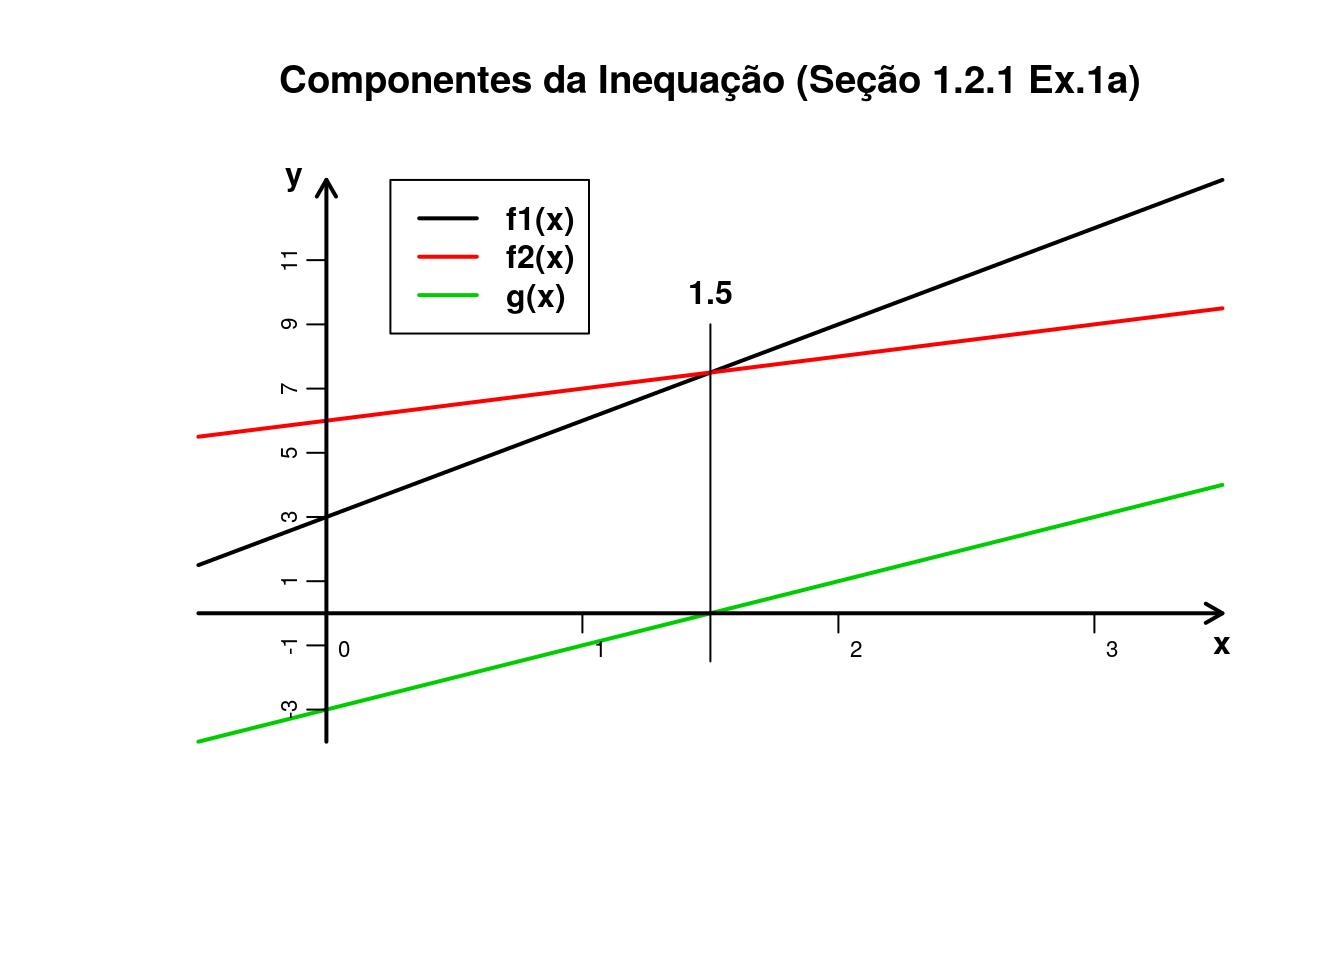
\includegraphics{Calculo-1_files/figure-latex/unnamed-chunk-4-1} \end{center}

\subsection{Exercícios Resolvidos}\label{exercicios-resolvidos}

\begin{enumerate}
\def\labelenumi{\arabic{enumi}.}
\item
  Resolva a inequação.

  \begin{enumerate}
  \def\labelenumii{\alph{enumii})}
  \tightlist
  \item
    \(3x+3 < x+6\)
  \end{enumerate}
\end{enumerate}

\begin{eqnarray}      
      3x+3 \ \ (-x) &<& x+6 \ \ (-x) \nonumber \\
      2x+3 &<& 6 \nonumber \\
      2x+3 \ \ (-3) &<& 6 \ \ (-3) \nonumber \\
      2x &<& 3 \nonumber \\
      \frac{2x}{2} &<& \frac{3}{2} \nonumber \\
      x &<& \frac{3}{2} \nonumber
\end{eqnarray}

\begin{Shaded}
\begin{Highlighting}[]
\CommentTok{# Resolução no R}

\NormalTok{##  Para resolver a inequação pelo R consideraremos as seguintes expressões:}
\NormalTok{## 'f1(x) = 3x + 3' e 'f2(x) = x + 6'.}
\NormalTok{f1 <-}\StringTok{ }\ControlFlowTok{function}\NormalTok{(x)\{}
  \DecValTok{3}\OperatorTok{*}\NormalTok{x }\OperatorTok{+}\StringTok{ }\DecValTok{3}
\NormalTok{\}}

\NormalTok{f2 <-}\StringTok{ }\ControlFlowTok{function}\NormalTok{(x)\{}
\NormalTok{  x }\OperatorTok{+}\StringTok{ }\DecValTok{6}
\NormalTok{\}}

\NormalTok{##  A desigualdade é 'f1(x) < f2(x)' logo 'f1(x) - f2(x) < 0'. Logo queremos os}
\NormalTok{## valores de x para os quais 'f1(x) - f2(x)' seja menor que zero.}
\NormalTok{##  Começaremos achando a raiz da expressão 'f1(x) - f2(x)'.}
\NormalTok{##  A função abaixo utiliza utiliza iterações para achar a raiz em um intervalo}
\NormalTok{## pré-determinado, utiliza-se aqui o intervalo (-10, 10) mas é possível inserir}
\NormalTok{## grandes intervalos a um certo custo de tempo computacional (neste caso}
\NormalTok{## razoável).}
\KeywordTok{uniroot}\NormalTok{(}\ControlFlowTok{function}\NormalTok{(x)\{}\KeywordTok{f1}\NormalTok{(x) }\OperatorTok{-}\StringTok{ }\KeywordTok{f2}\NormalTok{(x)\}, }\KeywordTok{c}\NormalTok{(}\OperatorTok{-}\DecValTok{10}\NormalTok{, }\DecValTok{10}\NormalTok{))}\OperatorTok{$}\NormalTok{root}
\end{Highlighting}
\end{Shaded}

\begin{verbatim}
## [1] 1.5
\end{verbatim}

\begin{Shaded}
\begin{Highlighting}[]
\NormalTok{##  O resultado revela somente a raiz da função. No entanto queremos saber onde}
\NormalTok{## se localizam os valores positivos e negativos da função.}
\NormalTok{##  Chamaremos nessa etapa a expressão 'f1(x) - f2(x)' de 'g(x)'.}
\NormalTok{g <-}\StringTok{ }\ControlFlowTok{function}\NormalTok{(x)\{}
  \KeywordTok{f1}\NormalTok{(x) }\OperatorTok{-}\StringTok{ }\KeywordTok{f2}\NormalTok{(x)}
\NormalTok{\}}

\NormalTok{##  Sabemos que a raiz da função 'g(x)' é 1.5, logo basta verificarmos os}
\NormalTok{## valores ao redor da raiz.}
\NormalTok{x <-}\StringTok{ }\KeywordTok{seq}\NormalTok{(}\DataTypeTok{from =} \DecValTok{1}\NormalTok{, }\DataTypeTok{to =} \DecValTok{2}\NormalTok{, }\DataTypeTok{by =} \FloatTok{0.1}\NormalTok{)}
\KeywordTok{data.frame}\NormalTok{(x, }\KeywordTok{g}\NormalTok{(x))}
\end{Highlighting}
\end{Shaded}

\begin{verbatim}
##      x g.x.
## 1  1.0 -1.0
## 2  1.1 -0.8
## 3  1.2 -0.6
## 4  1.3 -0.4
## 5  1.4 -0.2
## 6  1.5  0.0
## 7  1.6  0.2
## 8  1.7  0.4
## 9  1.8  0.6
## 10 1.9  0.8
## 11 2.0  1.0
\end{verbatim}

\begin{Shaded}
\begin{Highlighting}[]
\NormalTok{##  Pode-se observar que para valores menores que 1.5, g(x) assume valores}
\NormalTok{## negativos. Logo os valores de x que satisfazem a inequação são dados por}
\NormalTok{## 'x < 1.5'}

\CommentTok{# Exemplo Gráfico}

\NormalTok{##  O gráfico a seguir representa f1(x), f2(x) e g(x). Observe que para valores}
\NormalTok{## menores que 1.5 temos f1(x) < f2(x), para x = 1.5 temos f1(x) = f2(x) e para}
\NormalTok{## valores maiores que 1.5 temos f1(x) > f2(x).}

\NormalTok{##  Repare também que para valores menores que zero temos g(x) < 0, para x = 0}
\NormalTok{## temos g(x) = 0 e para valores maiores que zero temos g(x) > 0.}

\NormalTok{##  Curvas:}
\KeywordTok{curve}\NormalTok{(f1, }\DataTypeTok{from =} \OperatorTok{-}\DecValTok{2}\NormalTok{, }\DataTypeTok{to =} \DecValTok{4}\NormalTok{, }\DataTypeTok{xlim =} \KeywordTok{c}\NormalTok{(}\OperatorTok{-}\DecValTok{2}\NormalTok{, }\FloatTok{4.5}\NormalTok{), }\DataTypeTok{ylim =} \KeywordTok{c}\NormalTok{(}\OperatorTok{-}\DecValTok{3}\NormalTok{, }\DecValTok{16}\NormalTok{), }\DataTypeTok{lwd =} \DecValTok{2}\NormalTok{,}
      \DataTypeTok{bty =} \StringTok{'n'}\NormalTok{, }\DataTypeTok{xaxt =} \StringTok{'n'}\NormalTok{, }\DataTypeTok{yaxt =} \StringTok{'n'}\NormalTok{, }\DataTypeTok{ylab =} \StringTok{''}\NormalTok{, }\DataTypeTok{xlab =} \StringTok{''}\NormalTok{,}
      \DataTypeTok{main =} \StringTok{'Componentes da Inequação'}\NormalTok{)}
\KeywordTok{curve}\NormalTok{(f2, }\DataTypeTok{from =} \OperatorTok{-}\DecValTok{2}\NormalTok{, }\DataTypeTok{to =} \DecValTok{4}\NormalTok{, }\DataTypeTok{add =} \OtherTok{TRUE}\NormalTok{, }\DataTypeTok{col =} \DecValTok{2}\NormalTok{, }\DataTypeTok{lwd =} \DecValTok{2}\NormalTok{)}
\KeywordTok{curve}\NormalTok{(g, }\DataTypeTok{from =} \OperatorTok{-}\DecValTok{2}\NormalTok{, }\DataTypeTok{to =} \DecValTok{4}\NormalTok{, }\DataTypeTok{add =} \OtherTok{TRUE}\NormalTok{, }\DataTypeTok{col =} \DecValTok{3}\NormalTok{, }\DataTypeTok{lwd =} \DecValTok{2}\NormalTok{)}

\NormalTok{##  Eixos:}
\KeywordTok{arrows}\NormalTok{(}\DataTypeTok{x0 =} \OperatorTok{-}\FloatTok{2.5}\NormalTok{, }\DataTypeTok{x1 =} \DecValTok{4}\NormalTok{,}
       \DataTypeTok{y0 =} \DecValTok{0}\NormalTok{, }\DataTypeTok{y1 =} \DecValTok{0}\NormalTok{, }\DataTypeTok{lwd =} \DecValTok{2}\NormalTok{, }\DataTypeTok{length =} \FloatTok{0.1}\NormalTok{)}
\KeywordTok{arrows}\NormalTok{(}\DataTypeTok{x0 =} \DecValTok{0}\NormalTok{, }\DataTypeTok{x1 =} \DecValTok{0}\NormalTok{,}
       \DataTypeTok{y0 =} \OperatorTok{-}\DecValTok{4}\NormalTok{, }\DataTypeTok{y1 =} \DecValTok{15}\NormalTok{, }\DataTypeTok{lwd =} \DecValTok{2}\NormalTok{, }\DataTypeTok{length =} \FloatTok{0.1}\NormalTok{)}

\NormalTok{##  Ponto de intersecção:}
\KeywordTok{segments}\NormalTok{(}\DataTypeTok{x0 =} \FloatTok{1.5}\NormalTok{, }\DataTypeTok{x1 =} \FloatTok{1.5}\NormalTok{,}
         \DataTypeTok{y0 =} \OperatorTok{-}\DecValTok{2}\NormalTok{, }\DataTypeTok{y1 =} \DecValTok{10}\NormalTok{, }\DataTypeTok{lwd =} \DecValTok{1}\NormalTok{)}

\NormalTok{##  Enumeração dos eixos:}
\KeywordTok{axis}\NormalTok{(}\DataTypeTok{side =} \DecValTok{1}\NormalTok{, }\KeywordTok{c}\NormalTok{(}\KeywordTok{seq}\NormalTok{(}\OperatorTok{-}\DecValTok{2}\NormalTok{, }\OperatorTok{-}\DecValTok{1}\NormalTok{, }\DecValTok{1}\NormalTok{), }\KeywordTok{seq}\NormalTok{(}\DecValTok{1}\NormalTok{, }\DecValTok{3}\NormalTok{, }\DecValTok{1}\NormalTok{)), }\DataTypeTok{pos =} \DecValTok{0}\NormalTok{)}
\KeywordTok{axis}\NormalTok{(}\DataTypeTok{side =} \DecValTok{2}\NormalTok{, }\KeywordTok{c}\NormalTok{(}\OperatorTok{-}\DecValTok{3}\NormalTok{, }\DecValTok{3}\NormalTok{, }\DecValTok{6}\NormalTok{, }\DecValTok{9}\NormalTok{, }\DecValTok{12}\NormalTok{), }\DataTypeTok{pos =} \DecValTok{0}\NormalTok{)}

\NormalTok{##  Legenda:}
\KeywordTok{legend}\NormalTok{(}\OperatorTok{-}\FloatTok{2.25}\NormalTok{, }\DecValTok{13}\NormalTok{, }\DataTypeTok{col =} \KeywordTok{c}\NormalTok{(}\DecValTok{1}\NormalTok{, }\DecValTok{2}\NormalTok{, }\DecValTok{3}\NormalTok{), }\KeywordTok{c}\NormalTok{(}\StringTok{'f1(x)'}\NormalTok{, }\StringTok{'f2(x)'}\NormalTok{, }\StringTok{'g(x)'}\NormalTok{),}
       \DataTypeTok{lwd =} \DecValTok{2}\NormalTok{, }\DataTypeTok{text.font =} \DecValTok{2}\NormalTok{)}

\KeywordTok{text}\NormalTok{(}\DataTypeTok{x =} \KeywordTok{c}\NormalTok{(}\FloatTok{4.15}\NormalTok{, }\DecValTok{0}\NormalTok{, }\OperatorTok{-}\FloatTok{0.2}\NormalTok{, }\FloatTok{1.5}\NormalTok{), }\DataTypeTok{y =} \KeywordTok{c}\NormalTok{(}\DecValTok{0}\NormalTok{, }\FloatTok{15.75}\NormalTok{, }\OperatorTok{-}\DecValTok{1}\NormalTok{, }\DecValTok{11}\NormalTok{),}
     \DataTypeTok{labels =} \KeywordTok{c}\NormalTok{(}\StringTok{"x"}\NormalTok{, }\StringTok{"y"}\NormalTok{, }\StringTok{"0"}\NormalTok{, }\StringTok{"1.5"}\NormalTok{), }\DataTypeTok{font =} \DecValTok{2}\NormalTok{)}
\end{Highlighting}
\end{Shaded}

\begin{center}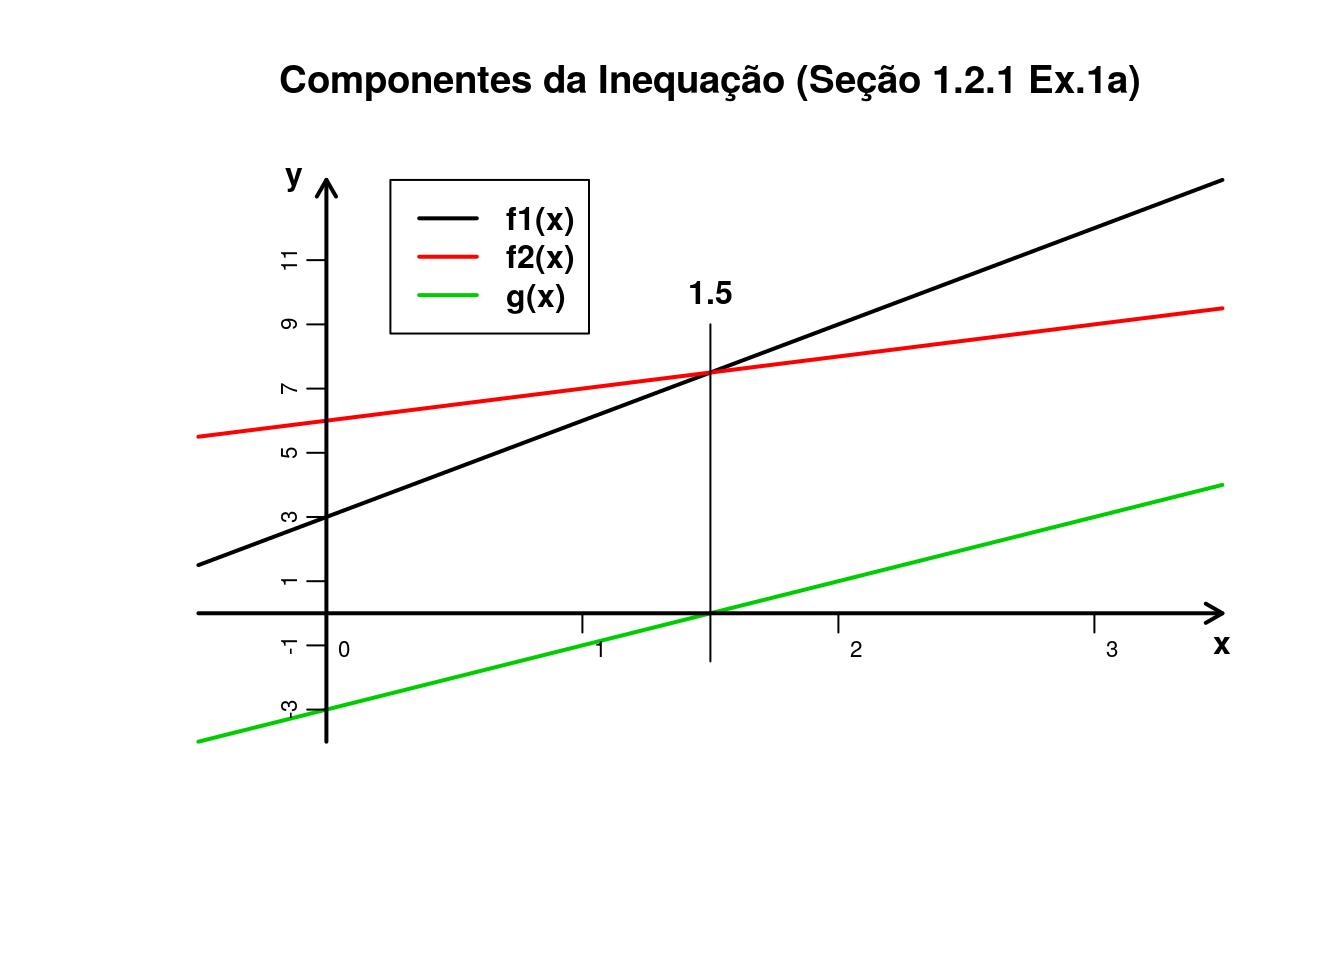
\includegraphics{Calculo-1_files/figure-latex/unnamed-chunk-5-1} \end{center}

\chapter{Sem Título}\label{sem-titulo}

\chapter{Sem Título}\label{sem-titulo-1}

\chapter{Sem Título}\label{sem-titulo-2}

\chapter{Sem Título}\label{sem-titulo-3}

\bibliography{book.bib,packages.bib}


\end{document}
